\documentclass{tietreport}

\usepackage{graphicx}
\usepackage{float}
\usepackage{enumitem}
\usepackage{array}
\usepackage{tabularx}
\hypersetup{hidelinks}
\setlist{nosep}

% Course/Lab header
\TitlePageHeader{%
  UCS503P - Software Engineering Project%
}

% Main project title
\ProjectTitle{%
  Sortify: AI-Powered Waste Identification and Disposal Guidance%
}

% Subtitle or project description
\ProjectSubTitle{%
  Prototype Stage Report%
}

% Student information
\author{%
  \texttt{1024160015} Daksh Aggarwal, CSED \\
  \texttt{1024160002} Mankirat Singh, CSED \\
  \texttt{1024160028} Saket Gatyan, CSED%
}

% Degree, year, program
\TitlePageSubText{%
  BE, Computer Science and Engineering Department%
}

% Faculty advisor/guide name
\AdvisorName{%
  Dr. Jeelani Asif%
}

% Evaluation period and department info
\TitlePageFooterText{{%
    \large Prototype Stage Evaluation \\[0.2cm]
    \bfseries Computer Science and Engineering Department%
  } \\[0.15cm]
  Thapar Institute of Engineering and Technology,
  Patiala%
}

\begin{document}

\maketitle
\tableofcontents

\chapter{Introduction}

\section{Background and Context}

Sortify is a mobile-first waste identification and disposal guidance system. The higher-order goal stated for the project is to reduce uncertainty at the point where a user decides how to dispose of an item. The system is intended to help users move from an unidentified waste item to actionable disposal instructions instead of only providing a raw classification label.

The current prototype focuses on demonstrating the user-facing workflow through a React Native mobile application. It presents a working local demo of scanning, sample prediction results, a searchable waste guide, saved history, feedback submission, a scripted assistant, profile settings, and a demo administrative interface. The prototype does not yet connect to a deployed backend service or a trained image-classification model.

\section{Problem Statement}

Users often encounter everyday items whose disposal route is unclear. The project proposal identifies common pain points such as uncertainty about waste categories, fragmented disposal information, incorrect segregation, lack of actionable guidance, and location-dependent disposal rules.

The prototype addresses this problem at the interface level by making disposal guidance visible immediately after a demo scan or manual catalog selection. It also shows how the user can save results, review them later, ask item-specific questions, and submit corrections when a result appears wrong.

\section{Prototype Objectives}

The prototype-stage work completed so far demonstrates the following implemented objectives:

\begin{enumerate}[leftmargin=0.7cm]
  \item Build a mobile application shell with navigation between Sortify's main user-facing screens.
  \item Implement a local waste catalog covering the proposed waste streams: recyclable, organic, general waste, e-waste, and hazardous waste.
  \item Demonstrate a scan-to-result workflow using selectable demo samples and simulated confidence values.
  \item Provide actionable disposal steps, caution notes, and local guidance text for catalog items.
  \item Support local history, profile settings, feedback, assistant messages, and catalog edits using device-local storage.
\end{enumerate}

\chapter{Methodology and Design}

\section{System Design Reference}

The project proposal defines Sortify as a system combining a mobile application, ML-based identification, a structured waste knowledge base, location-aware guidance, history, feedback, administrative tools, and a conversational assistant. At the prototype stage, the implemented system is a local mobile demo that models these interactions without claiming live backend, database, or ML deployment.

\begin{figure}[htbp]
  \centering
  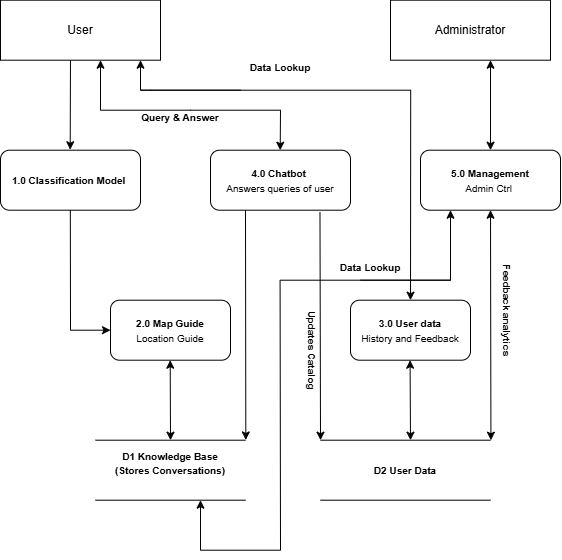
\includegraphics[width=0.76\textwidth]{../docs/diagrams/data_flow_diagram/level1.png}
  \caption{Level-1 Data Flow Diagram for Sortify}
  \label{fig:level1-dfd}
\end{figure}

\section{Functional Flow}

The implemented demo follows the core proposal workflow in prototype form:

\begin{enumerate}[leftmargin=0.7cm]
  \item The user opens the app and navigates to the scan screen.
  \item The user either selects a sample item or uploads/captures a photo.
  \item For uploaded or captured photos, the prototype asks the user to choose the demo result; the actual image is not sent to a backend.
  \item The app simulates prediction processing and opens a result screen with a demo confidence value.
  \item The result screen shows item category, material, disposal steps, caution notes where available, and local guidance text.
  \item The user can save the item, mark it as sorted, submit a correction, ask the assistant about the item, or return to the guide.
\end{enumerate}

\begin{figure}[htbp]
  \centering
  
\includegraphics[width=0.66\textwidth]{../docs/diagrams/activity_diagram/activity.png}
  \caption{Activity Diagram for the Sortify Workflow}
  \label{fig:activity-diagram}
\end{figure}

\section{Use Cases Represented in the Prototype}

The implemented prototype currently represents the standard user flow and an open demo administrator flow. Users can search the guide, run a simulated scan, inspect disposal guidance, save results, review history, ask the assistant, manage local profile data, and submit corrections. The admin screen supports catalog edits, feedback review, and prototype usage summaries.

\begin{figure}[htbp]
  \centering
  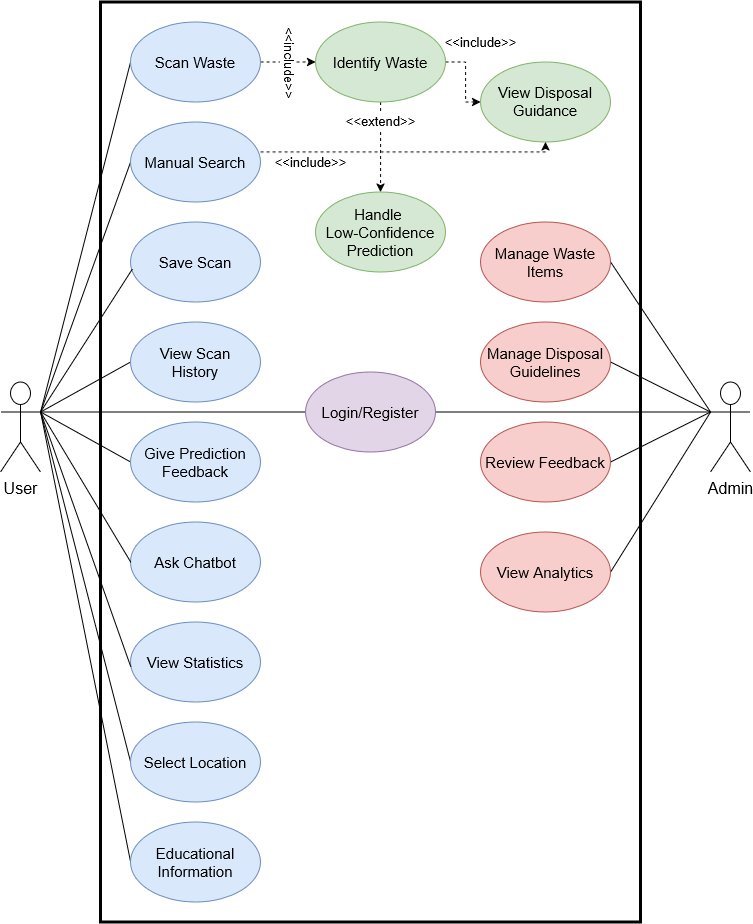
\includegraphics[width=0.58\textwidth]{../docs/diagrams/use_case_diagram/use_case_diagram.png}
  \caption{Use Case Diagram for Sortify}
  \label{fig:use-case-diagram}
\end{figure}

\section{Data Model Reference}

The prototype uses local application state rather than a production database. The data represented in the app includes waste items, scans, feedback, profile data, assistant messages, and the selected location. This aligns with the entities expected for a fuller system while remaining limited to device-local demo storage.

\begin{figure}[htbp]
  \centering
  
\includegraphics[width=0.68\textwidth]{../docs/diagrams/er_diagram/er.png}
  \caption{Entity Relationship Diagram for Sortify}
  \label{fig:er-diagram}
\end{figure}

\section{Technical Stack Implemented}

The implemented demo is built as an Expo/React Native application using TypeScript. It uses Expo Router for navigation, Expo Image Picker for camera and image-library access, React Native components for the interface, and AsyncStorage for local persistence. The current prototype is frontend-only and does not include a connected FastAPI backend, PostgreSQL database, PyTorch model, or live LLM-based assistant.

\chapter{Implemented Prototype Features}

\section{Application Navigation and Layout}

The application has routed screens for Home, Waste Guide, Scan, Activity, History, Assistant, Learn, Profile, Admin, and Result. On iOS, the app uses native tabs. On other platforms, it uses a custom shell around the routed screens.

The Home screen greets the user when a local demo profile exists, provides a primary action to scan an item, and shows progress summaries and milestone information based on locally saved scans.

\section{Waste Catalog and Guide}

The prototype includes a structured local catalog of waste items. Each catalog entry stores an item name, waste category, material, description, disposal steps, optional caution text, and searchable keywords.

Implemented guide functionality includes:

\begin{itemize}[leftmargin=0.7cm]
  \item Searching by item name, material, or keyword.
  \item Filtering by category: recyclable, organic, general waste, e-waste, and hazardous.
  \item Pagination of catalog results.
  \item Opening an item result page from the guide.
\end{itemize}

The initial catalog includes examples such as plastic bottle, banana peel, cardboard box, household battery, glass jar, aluminium can, vegetable scraps, used tissue, snack wrapper, phone charger, old headphones, expired medicine, newspaper, dry leaves, and broken ceramic mug.

\section{Scan Demo}

The scan screen implements two modes: photo and sample. In photo mode, the app can request camera permission, open the camera on supported platforms, open the image library, preview a selected image, reject images larger than 10 MB, and reject images smaller than 100 by 100 pixels.

The current identification step is simulated. The app lets the user choose a demo item and then opens the result screen after a short delay. The selected sample determines the result, and the app explicitly states that photos stay on the device.

The scan demo also includes two controlled scenarios:

\begin{itemize}[leftmargin=0.7cm]
  \item Low-confidence result, which sends a 46\% demo confidence value and asks the user to confirm before saving.
  \item Service unavailable, which shows an error state and suggests retrying or using the waste guide.
\end{itemize}

\section{Result and Disposal Guidance}

The result screen shows the selected item name, material, category badge, and demo confidence when available. It displays numbered disposal steps and caution notes for items that require extra care.

Implemented result actions include:

\begin{itemize}[leftmargin=0.7cm]
  \item Save the item to local history.
  \item Mark the item as sorted.
  \item View local guidance text based on the selected location and waste category.
  \item Ask the assistant about the current item.
  \item Submit a correction when the result appears wrong.
\end{itemize}

The location guidance is implemented as generated local text. It does not connect to verified local schedules or collection-point services.

\section{History and Activity}

The history screen lists saved scans and supports searching, filtering by sorted status, pagination, opening a saved result, and removing an item from history. Saved scans store item ID, date, confidence, source, and sorted status.

The activity screen summarizes locally saved activity. It includes a seven-day saved-item bar view and a category breakdown using the waste categories in the catalog. These summaries are based only on local demo data.

\section{Profile and Local Data Settings}

The profile screen implements a local demo account flow. Users can create or enter a demo account using name, email, and a password field. The password is validated for length during the demo flow but is not stored or verified. The profile stores only the user's name and email locally.

The data and privacy section explains the local storage behavior and provides a reset action that clears local activity and restores the original guide data.

\section{Scripted Assistant}

The assistant screen implements a catalog-grounded scripted demo. Users can ask item-related questions, and the app matches words against catalog keywords. If it finds a catalog item, it returns the item category, disposal steps, caution note if present, and a reminder to check accepted materials locally.

The assistant also supports item context from a result screen, follow-up-style questions, conversation persistence in local storage, and clearing the local conversation. It is not connected to a live LLM or RAG backend in the current prototype.

\section{Admin Demo}

The admin screen is implemented as an open-access demo area. It includes three sections:

\begin{itemize}[leftmargin=0.7cm]
  \item \textbf{Waste catalog:} search catalog entries, add a new item, edit existing guidance, select a category, edit three disposal steps, add an optional safety note, and delete an item.
  \item \textbf{Feedback:} review corrections submitted from result screens and toggle their status between pending and reviewed.
  \item \textbf{Analytics:} view local counts for waste items, saved discoveries, feedback to review, demo predictions saved, manual selections saved, corrections submitted, and corrections reviewed.
\end{itemize}

The analytics section explicitly avoids fabricating model-performance values. It notes that accuracy, F1 score, inference latency, and confusion matrix results require a trained model and held-out evaluation set.

\chapter{Results and Evaluation}

\section{Prototype Status}

The current implementation successfully demonstrates the frontend behavior of the core Sortify experience. The demo proves the app structure, navigation, catalog-driven guidance, local persistence, history flow, correction flow, assistant mockup, and admin catalog-management workflow.

\section{Implemented Versus Not Yet Implemented}

\begin{table}[htbp]
\centering
\small
\renewcommand{\arraystretch}{1.15}
\begin{tabularx}{\textwidth}{|>{\raggedright\arraybackslash}p{0.30\textwidth}|>{\raggedright\arraybackslash}X|}
  \hline
  \textbf{Area} & \textbf{Prototype status} \\
  \hline
  Mobile app UI & Implemented as an Expo/React Native TypeScript demo. \\
  \hline
  Image capture/upload & Implemented through Expo Image Picker with basic image validation. \\
  \hline
  ML prediction & Simulated using selected demo samples and confidence values. No trained model is connected. \\
  \hline
  Waste guide & Implemented as a local searchable and filterable catalog. \\
  \hline
  Disposal guidance & Implemented through catalog disposal steps, caution notes, and generated local guidance text. \\
  \hline
  History and activity & Implemented using local scan records and local summary views. \\
  \hline
  Feedback & Implemented locally through correction submission and admin review status. \\
  \hline
  Assistant & Implemented as a scripted keyword-based catalog demo, not live AI. \\
  \hline
  Admin dashboard & Implemented as an open demo for catalog editing, feedback review, and local analytics. \\
  \hline
  Backend, database, deployment & Not implemented in the current prototype. \\
  \hline
\end{tabularx}
\caption{Prototype implementation status}
\label{tab:prototype-status}
\end{table}

\section{Current Evaluation Limits}

The prototype is not ready for ML performance evaluation because it does not include a trained model, inference service, held-out dataset, or real prediction pipeline. Therefore, no accuracy, F1 score, confusion matrix, or inference-latency claims are made in this report.

The meaningful evaluation at this stage is functional: whether the implemented demo screens allow a user to complete the local scan-to-guidance workflow, search the catalog, save and review results, submit corrections, and manage catalog entries through the demo admin interface.

\chapter{Conclusion}

\section{Summary of Work}

The prototype stage delivers a functional local mobile demo for Sortify. It implements the frontend flow for scanning an item through simulated predictions, viewing disposal guidance, searching the waste guide, saving history, tracking activity, using a local demo profile, asking a scripted catalog-based assistant, submitting corrections, and managing guide entries in an admin demo.

The implemented work remains aligned with the proposal's emphasis on actionable disposal guidance. At the current stage, the app demonstrates the user experience and data flow, while backend integration, trained ML inference, production authentication, a real database, live location services, and a live conversational AI backend remain outside the implemented prototype.

\section{Next Work Based on Proposal Scope}

The next implementation steps should focus on replacing simulated parts with real services: connecting a FastAPI backend, integrating a trained image-classification model, moving local catalog and scan records to a proper database, adding authenticated user accounts, and validating the system with representative waste items.

\end{document}
